\section{Learning}
\noindent
The first part of the practical course was dedicated to learning the main control practices and hardware features of the dsPIC digital signal controllers from Microchip, widely used in embedded applications and robotics.\\

\noindent
\textbf{Developed skills}
\begin{itemize}
    \item extracting relevant information from datasheets
    \item expressing it in C language
    \item cross-compiling
    \item debugging (using Simulation environment)
\end{itemize}

\noindent
In the following section we introduce the most important aspects of each hardware peripheral of the microcontroller. For more details refer to dsPIC overview document \cite{alex}.\\
Please refer to the software section of the report to have more details about the peripheral’s settings used for our robot.

\subsection{Digital I/O}

The general purpose I/O (GPIO) pins allow the microcontroller to monitor and control other devices. Many pins are shared between several peripherals and the GPIO pins. An output multiplexer allows the peripheral to direct its outputs to the pin when the peripheral is enabled. Otherwise, the port is controlled by the I/O logic as shown in the figure \ref{fig:gpio} below.\\

\begin{figure}[H]
    \centering
    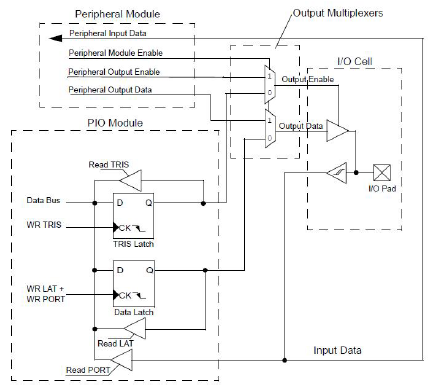
\includegraphics[width=0.5\textwidth]{figures/software/GPIO.PNG}
    \caption{Shared port structure \cite{alex}}
    \label{fig:gpio}
\end{figure}

\noindent
All port pins have three Special Function Registers (SFR), registers that control various aspects of the microprocessor's function, directly associated with the operation of the port pin:
\begin{itemize}
    \item \textbf{TRIS}\\
    The TRI-State Register sets the direction of the pin. The value ``1'' corresponds to an input pin and ``0'' to an output pin.\\
    The direction needs to be set before reading or writing the data from the ports. \\
    Only pins configured as digital can be used as input or output pins. Pins configured as analog must be used as input pin.
    \item \textbf{LAT}\\
    It sets the output value of the pin and returns the logic state of the output latch.
    \item \textbf{PORT}\\
    It returns the logic state of the pin. 
\end{itemize}
To avoid Read-Modify-Write issue, we always read from the port and write to the latch.\\

\noindent
\textit{Read-Modify-Write issue:}

\noindent
Since pins are grouped in port categories, in order to change a pin value, it is required to first load the port register in ALU, change the value with bit operations using a specific mask value and finally write the result into the port register. If there is not a long delay between two write instructions on the same port, the second operation may overwrite the first due to propagation delay. This issue is not encountered when writing on latch write since we read directly from the latch register. 

\subsection{Interrupts}

Interrupts are mechanisms that allow the microcontroller to react to external and internal events.\\
When the microcontroller receives an interrupt request (IRQ), it jumps to the interrupt service routine (ISR), executes it and returns back to the main program. 
Consequently, interrupts enable a quick reaction and are efficient for asynchronous events as they allow the microcontroller to allocate its maximum processing time for other tasks by avoiding redundant checking tasks.\\

\noindent
To be signalled to the CPU by the interrupt controller, the interrupt must be enabled and have a priority higher than the current CPU priority.\\
The natural priority is considered when two interrupts with the same assigned priority would occur simultaneously. This priority is linked to their position in the vector table.(refer to MCU datasheet table 7-1\cite{mcu})

\subsection{Timer}\label{subsec:timer}

\begin{figure}[H]
    \centering
    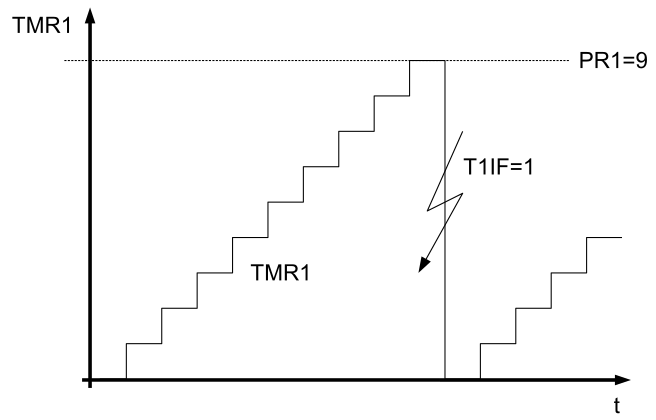
\includegraphics[width=0.5\textwidth]{figures/software/t1_demo.png}
    \caption{Principle of the Timer 1 \cite{alex}}
    \label{fig:t1_demo}
\end{figure}

Timers are used to measure the time or generate the accurate time delay using a binary counter that can be configured to count clock pulses. As seen in figure \ref{fig:t1_demo}, once it reaches the maximum set value, it rolls back to zero setting up an overflow flag and generates the interrupt if enabled. \\

\noindent
To generate the range of delays, we must set the maximum count value using the following formulas:\\
We first multiply the cycle period by a prescaler, to deduce the time between two increments of the counter:
$$tick=prescaler*T_{CY}$$
Then we derive the maxcount which we store inside our period register (PR):
$$maxcount=Timer delay/tick$$

\noindent
If we did not use a prescaler, the maximum time we could set between T1 interrupts would be $T_{CY}*(2^{16}-1)$. But since we can use a prescaler, we only count for example every second or fourth clock cycle depending on our prescaler. This allows us to wait twice or four times the amount of time.

Depending on our application, we choose a different prescaler:
\begin{enumerate}
    \item If we need a high timer resolution, the smallest prescaler value should be chosen. 
    \item If we do not care about the resolution, the highest prescaler value should be chosen. Errors in the time period relative to the period itself would be smaller with a longer period (in our case: a larger prescaler causes a longer period).
\end{enumerate}

\subsection{Pulse Width Modulation} 

\noindent
Pulse width modulation (PWM) is the method of choice to control the amount of energy that is supplied to an actuator, light source or any other device when employing digital control systems.\\
The duty cycle is defined as the proportion of time the PWM output is switched on with respect to the PWM period.
The PWM period ($T_{PWM}$) is fixed and represents the cycle time of the signal.

\noindent
As seen in figure \ref{fig:pwm_demo}, we can vary the duty cycle by changing the time that the PWM output is switched on ($T_{DC}$).

$$DC = \frac{T_{DC}}{T_{PWM}}$$

\begin{figure}[H]
    \centering
    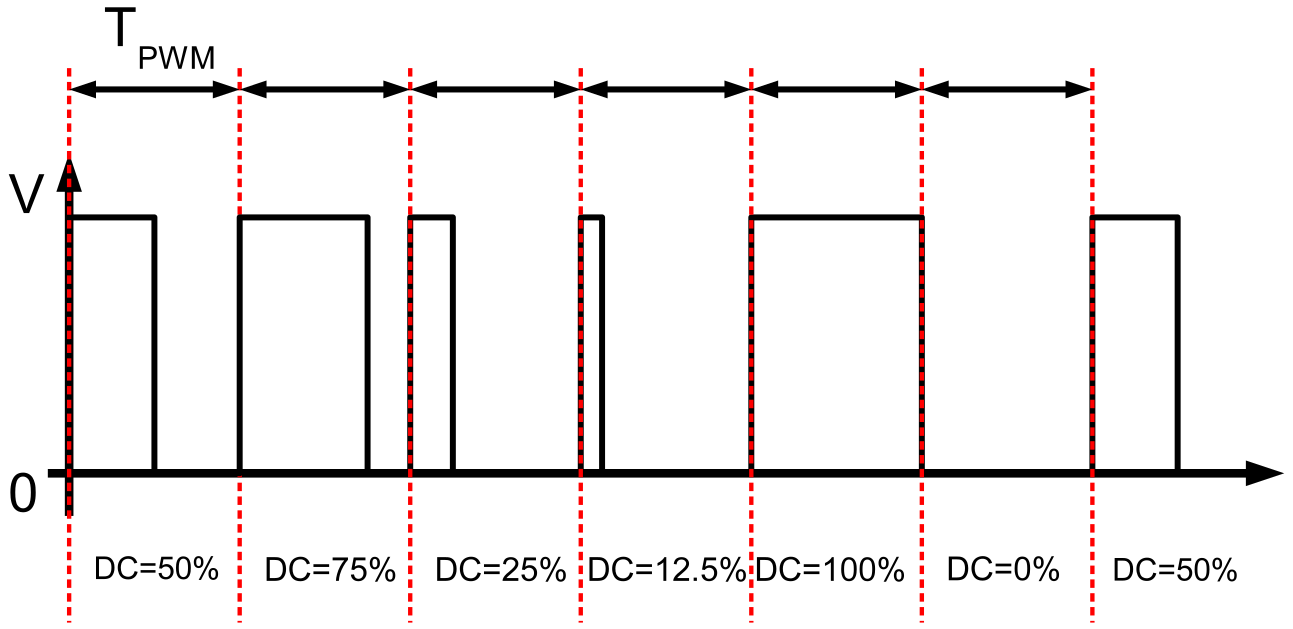
\includegraphics[width=0.5\textwidth]{figures/software/pwm_demo.png}
    \caption{Principle of PWM \cite{alex}}
    \label{fig:pwm_demo}
\end{figure}

\begin{figure}[H]
    \centering
    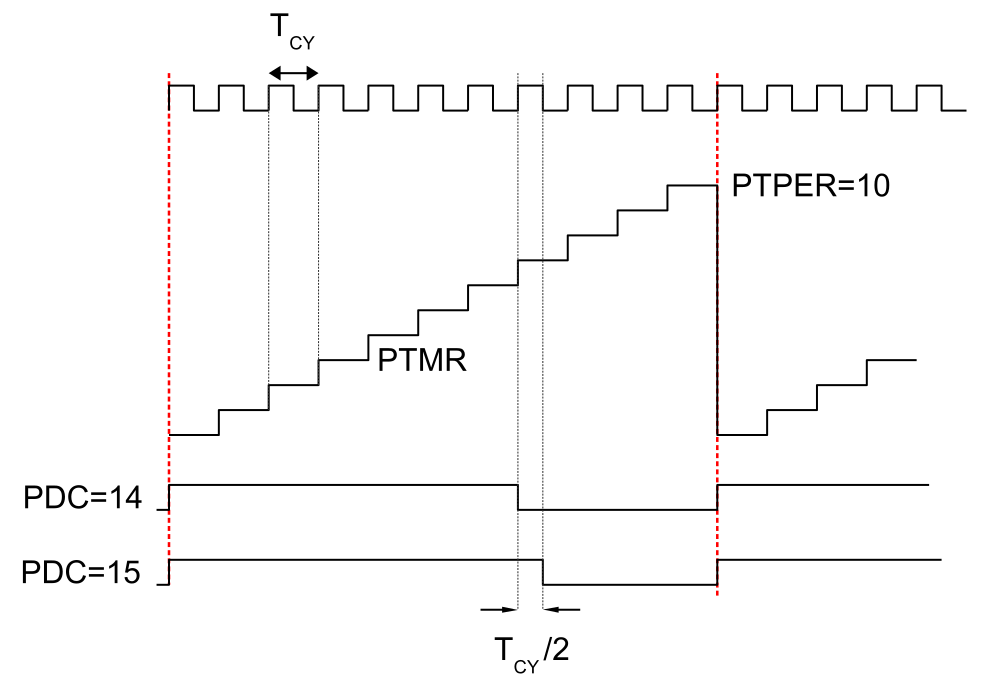
\includegraphics[width=0.5\textwidth]{figures/software/pwm_choice.png}
     \caption{Resolution of a PWM duty cycle \cite{alex}}
    \label{fig:pwm_choice}
\end{figure}

\noindent
The PWM frequency is application dependent. However, we should keep in mind that high frequency requires very fast switches and may cause electromagnetic interference problems. Whereas, low frequency causes the load to follow the pulse.\\
For driving a motor, a typical value would range between 5kHz and 50kHz, but for an accurate value we should consider the mechanical time constant and the electrical time constant of the motor.


The main elements of a PWM generator are a timer/counter and a comparator whose output drives the PWM signal. At the beginning of the cycle, the PWM signal is switched on. The comparator compares the timer/counter value with the duty cycle value ($PDC$). When this value is reached, the PWM output is switched off. The counter continues to increase until it reaches the PWM period value ($PTPER$) and then resets, completing one PWM period (see figure \ref{fig:pwm_choice}).

PWM period:
$$T_{PWM}=T_{CY}*(PTPER+1)*PTMR Prescale Value$$

DC: 
$$DC=100* \frac{PDC}{(2*(PTPER+1)}$$


\subsection{Universal Asynchronous Receiver Transmitter}

UART is the most commonly used protocol for asynchronous serial communication in microcontrollers due to its simplicity, easy implementation and minimum hardware requirements.\\

\begin{figure}[H]
    \centering
    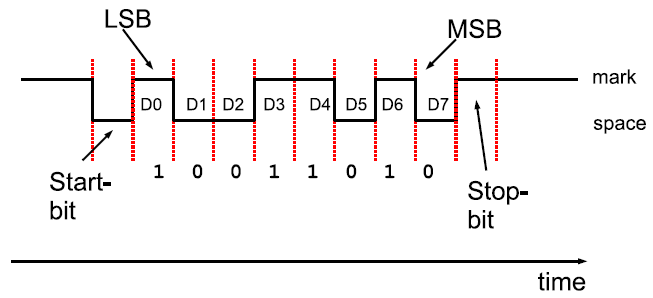
\includegraphics[width=0.5\textwidth]{figures/software/UART_com.PNG}
    \caption{UART transmission protocol\cite{alex}}
    \label{fig:uartProtocol}
\end{figure}

\noindent
As shown in figure \ref{fig:uartProtocol}, when no character is transmitted, the bus is typically logically high and transmission begins with the start bit which is logically low. After this, typically 8 data bits are transmitted and the transmission finishes with a logical high as a stop bit.\\

\noindent
To receive data from UART, we utilize a UART receive interrupt that will trigger every time a data packet is received in the UART receive registers (U1RXREG). This data is transferred to another variable and the receive buffer is cleared if full.


\noindent
The main criterion for UART communication is its baud rate, i.e. transmission speed. It is measured in bits per second and usually takes the following values: 9600bits/s, 28.8kbits/s, 57.6kbits/s.
This value is stored in U1/2BRG register and is derived from the clock cycle.
$$BaudRate = \frac{f_{CY}}{UnBRG+1}$$
For successful communication, both the device’s receiver and transmitter should be set to same baud rate.


\subsection{Quadrature Encoder Interface}

Quadrature encoders (also known as incremental encoders or optical encoders) are used for position and speed detection of rotating motion systems. They enable closed loop control of many motor control applications.
\vskip 0.2in
\noindent
The Quadrature Encoder module provides a simple interface to incremental optical encoders, which allows to obtain signed velocity using two photo-transistors that are offset by one quarter of the cycle period. It accepts the A, B and index connections from the incremental encoder and stores the accumulated count pulses in a dedicated 16-bit time base.

\begin{figure}[H]
    \centering
    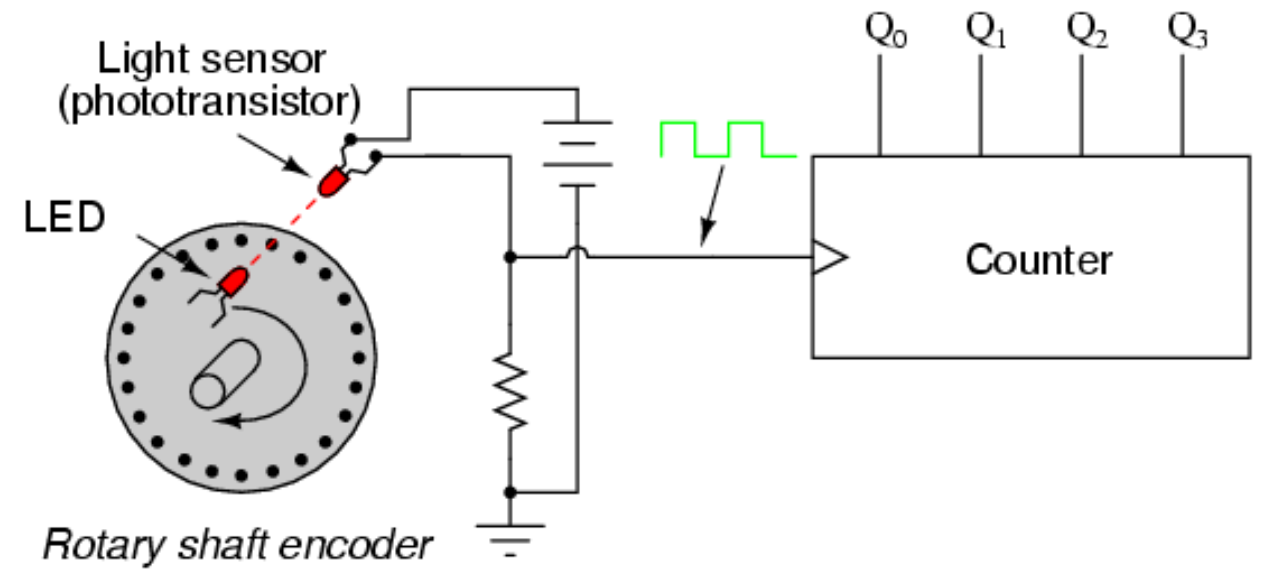
\includegraphics[width=0.5\textwidth]{figures/software/qei_demo.png}
    \caption{Principle of a Quadrature Encoder \cite{alex}}
    \label{fig:qei_demo}
\end{figure}
\vskip 0.2in
\noindent
Whenever the wheel is rotated, light emitted from the LED will hit the photo-transistor if there is a hole between them. Light sensor and emitter are separated by the wheel seen in figure \ref{fig:qei_demo}. The time passed between the phototransistor turning on after registering light and turning off again after the light disappears behind the wheel, will determine the velocity of our motor.
\vskip 0.2in
\noindent
The two channels, Phase A (QEA) and Phase B (QEB) enable to know the direction of the motor. If Phase A leads Phase B, then the direction of the motor is forward (counter is incremented). If Phase A lags Phase B then the direction of the motor is reverse (counter is decremented). A third channel, termed Index pulse, occurs once per revolution and is used as a reference to establish an absolute position.\\
However, the high resolution of the encoders leads rapidly to an overflow or underflow of the 16 bits counter register. To keep track of the total counts, a global variable should be updated accordingly at each interrupt call.

\subsection{Analog to Digital Converter}

Since we employ a digital microcontroller, it is necessary to convert the analog values from sensors to digital values. This is performed by the analog-to digital converters (ADC).\\
The ADC module converts a continuous time and value signal to a discrete time and value signal by sampling at a fixed sample period and converting the analog values into an integer values stored in a k-bits binary representation.

\vskip 0.2in
\noindent
During conversion the analog signal should be ``held'' constant throughout the process. This is usually done with a sample and hold circuit. It takes a ``snapshot'' of the input signal and stores it on the plates of a capacitor to have a steady signal. The acquisition time should be long enough for the capacitor to charge enough to match, as closely as possible, the incoming voltage.
\vskip 0.2in
\noindent
After the analog input is captured by the sample-and-hold (S/H) amplifier, it is compared with the output of a digital-to-analog converter to perform the conversion. refer to figure \ref{fig:sac} 
\vskip 0.2in
\noindent
DSPs have integrated ADCs, depending on the dsPIC type, they are either 10 bit or 12 bit ADCs.  The most commonly used ADCs are based on the successive approximation principle which uses a binary search to find each bit of the output voltage.\\

\begin{figure}[H]
    \centering
    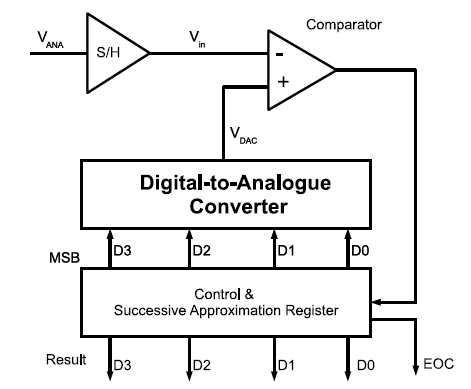
\includegraphics[width=0.5\textwidth]{figures/software/SAC.PNG}
    \caption{Successive Approximation Conversion principle\cite{alex}}
    \label{fig:sac}
\end{figure}
\noindent
ADC raises an interrupt when all the configured channels have been sampled. The results are available on the 16 16-bit ADC buffers (ADCBUF0, …, ADCUFF).


\subsection{Direct Memory Access}

Direct memory access (DMA) is the ability for an I/O device to transfer data directly to or from memory.  It can be seen as a co-processor that is used to quickly transfer data between main memory and peripherals without the intervention of the CPU. Hence, freeing up the CPU for more valuable tasks while the DMA controller takes care of the data movement and pointer incrementing.


\vskip 0.2in
\noindent
The dsPIC33 family has an integrated DMA controller optimized for high-performance, real-time, embedded applications. DMA uses a second bus master within the system and therefore, can continue to transfer data when the CPU has entered Idle mode.\\
When data is ready to be transferred from the peripheral, a DMA request is issued by the peripheral. When the block transfer is complete, the DMA channel issues an interrupt (if enabled).
\vskip 0.2in
\noindent
The DMA channel supports different operating modes:
\begin{itemize}
    \item Post-Increment or static DPSRAM addressing.
    \item Peripheral Indirect Addressing or Register Indirect Addressing.
    \item One-Shot or continuous block transfers.
    \item Ping-Pong mode (Auto-switch between two start addresses offsets (DMAxSTA or DMAxSTB) after each transfer complete)
\end{itemize}

\noindent
Please refer to the DMA section of the Family reference manual \cite{dma} for more details about these operating modes.


\subsection{Fusion Workshop}
For learning Autodesk Fusion 360, a one-day workshop was held. In this workshop, the basic aspects of CAD modelling and basic features of Fusion 360 were introduced, as well as more advanced features such as history timeline, version control, and collaboration between users.

One very helpful thing that we learned in the workshop is to import 3rd party parts. The 3D model of the motor that we are using is imported, such that a fitting motor mount can be designed very precisely and accurately according to the dimension of the motor. (Fig. \ref{fig:fusion_import})

We practiced using many “modeling” features, as well as “assembly” features such as joint, and changing “physical material” and “appearance” to create a box with a moving joint that can be opened and has varying appearances. Later the user collaboration feature was demonstrated using these boxes by assembling them on a table. (Fig. \ref{fig:fusion_collab_table})

\begin{figure}[htb]
    \centering
    \begin{minipage}{.45\textwidth}
          \centering
            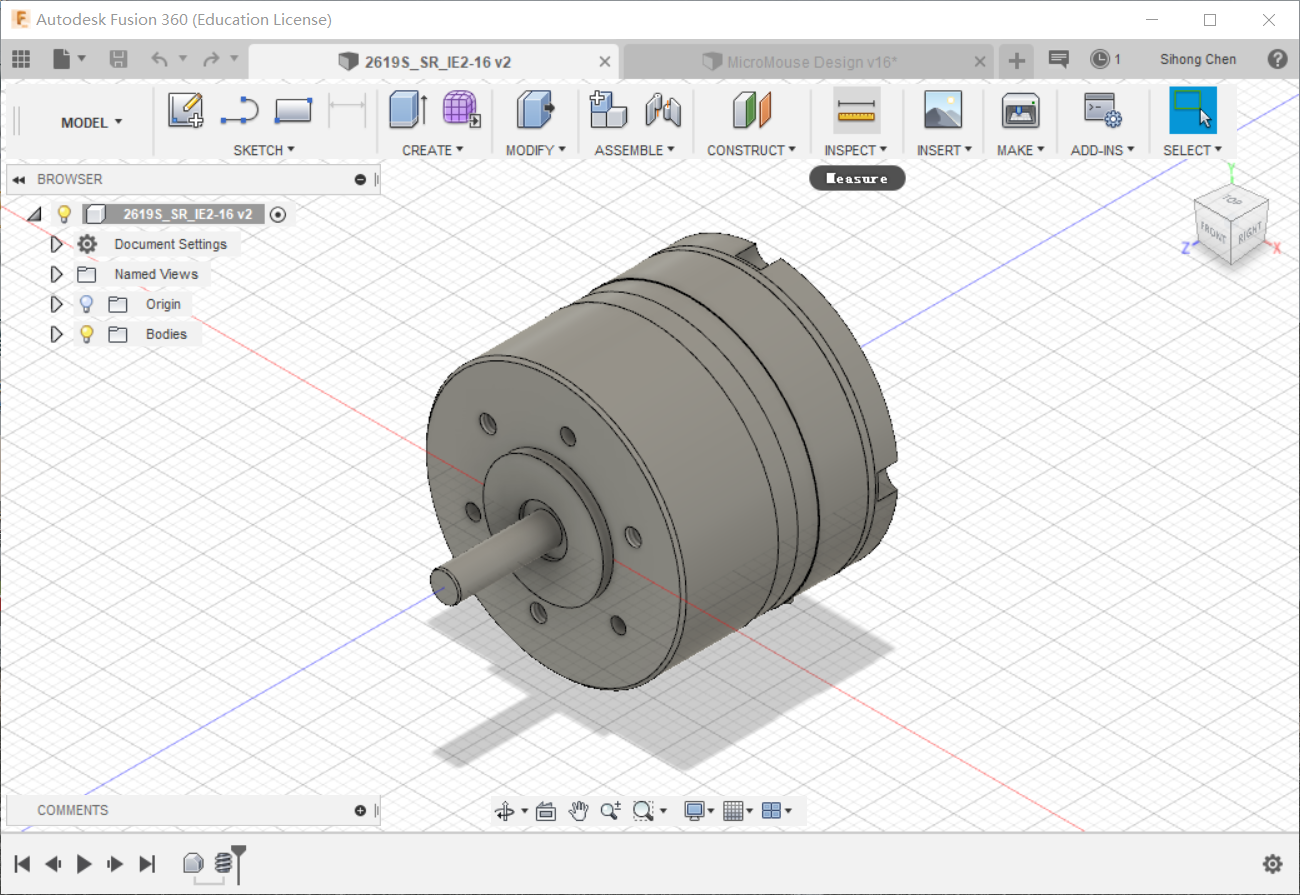
\includegraphics[width=.9\linewidth]{figures/Casing/FusionImport.PNG}
              \caption{Import 3D CAD Model from 3rd party}
                \label{fig:fusion_import}
    \end{minipage}
    \begin{minipage}{.45\textwidth}
          \centering
            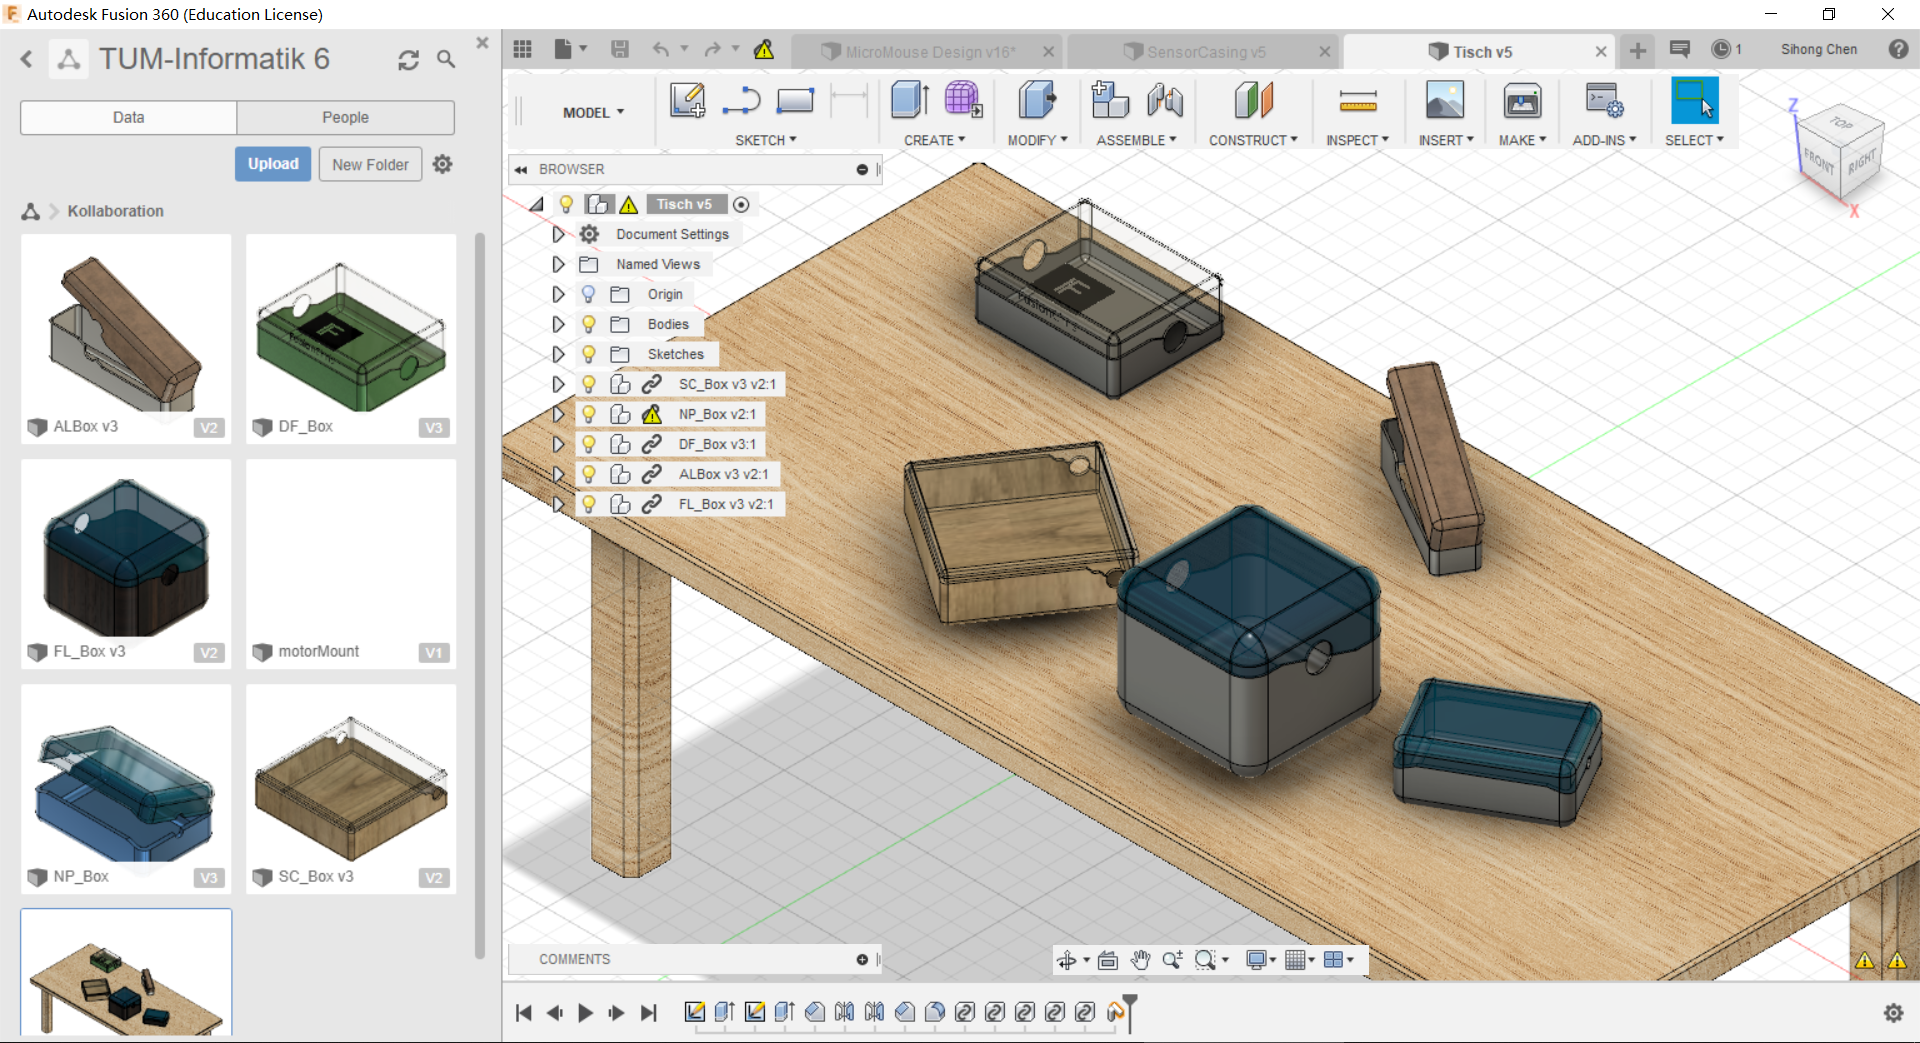
\includegraphics[width=.9\linewidth]{figures/Casing/FusionCollaborationTable.PNG}
              \caption{Individually made boxes put together on one table in Fusion collaboration}
                \label{fig:fusion_collab_table}
    \end{minipage}
\end{figure}

\noindent
In the workshop, a synchronisation feature between Autodesk EAGLE and Autodesk Fusion 360 is briefly introduced, which has the potential to reduce the back-and-forth process between CAD 3D model design and PCB design. However, in practice, we find that the lack of 3D models from the electronic components that we are using renders the usefulness of this feature somewhat limited.

In order to tackle some of the challenges we faced for designing the casing, some more advanced features of Fusion 360 have been utilised.

\noindent
One example is to set “parameter” values when creating the parts, which allowed easy modification to the model. This is helpful because our design processes are parallel to each other, and in the end the casing has to matched the physical dimension of the board. Therefore a back-and-forth process between PCB design and CAD design is unavoidable. The “parameter” feature in Fusion 360 accelerates this process and saves a lot of time and unnecessary work.

Furthermore the freeform and sculpting tool enables us to create more free flowing surfaces. This tool is traditionally reserved for industrial designers, and by combining this with the CAD solid modelling environment, Fusion 360 has partially earned its namesake: a fusion of different design processes. For our project, it enabled a more interesting look to the design.

\FloatBarrier
\vspace{1cm}


